\section{Method}
\label{sec:locvqa_locatt_method}

Our method extends a \gls{vqa} model to answer localized questions. We define a \emph{localized question} for an image~$\x$ as a tuple~$(\q, \m)$, where $\q$~is a question, and $\m$~is a binary mask of the same size as~$\x$ that identifies the region to which the question pertains. Our \gls{vqa} model, parameterized by $\bm{\theta}$ and depicted in Fig.~\ref{fig:method_locvqa}, accepts an image and a localized question as input and produces a probability distribution over a finite set~$\mathcal{A}$ of possible answers. The final answer~$\hat{a}$ of the model is the element with the highest probability,
\begin{equation}
    \hat{a} = \argmax_{a\in\mathcal{A}} p(a\mid \q, \x, \m; \bm{\theta}).
\end{equation}
The model proceeds in three stages to produce its prediction: input embedding, localized attention, and final classification.

\subsection{Input Embedding} The question~$\q$ is first processed by an \gls{lstm}~\cite{hochreiter1997long} to produce an embedding~$\hat{\q}\in\real^Q$. Similarly, the image~$\x$ is processed by a ResNet-152~\cite{he2016deep} to produce the feature map~$\hat{\x}\in\real^{C\times{}H\times{}W}$.

\subsection{Localized Attention} An attention mechanism uses the embedding to determine relevant parts of the image to answer the corresponding question. Unlike previous attention methods, we include the region information that the mask defines. Our \emph{localized attention} module (Fig.~\ref{fig:method_locvqa} right) uses both descriptors and the mask to produce multiple weighted versions of the image feature map,~$\hat{\x}'=\att(\hat{\q}, \hat{\x}, \m)$. To do so, the module first computes an attention map~$\g\in\real^{G\times{}H\times{}W}$ with $G$~glimpses by applying unmasked attention~\cite{kim2016hadamard,vu2020question} to the image feature map and the text descriptor. The value of the attention map at location~$(h, w)$ is computed as,
\begin{equation}
    \g_{:hw} = \textrm{softmax}\left(\W^{(g)}\cdot\textrm{ReLU}\left(\W^{(x)}\hat{\x}_{:hw} \odot \W^{(q)}\hat{\q}\right)\right),
\end{equation}
where the index ${:}hw$ indicates the feature vector at location~$(h, w)$, $\W^{(x)}\in\real^{C'\times C}$, $\W^{(q)}\in\real^{C'\times Q}$, and $\W^{(g)}\in\real^{G\times C'}$ are learnable parameters of linear transformations, and $\odot$~is the element-wise product. In practice, the transformations $\W^{(x)}$ and $\W^{(g)}$ are implemented with $1\times{}1$~convolutions and all linear transformations include a dropout layer applied to its input. The image feature maps~$\hat{\x}$ are then weighted with the attention map and masked with~$\m$ as,
\begin{equation}
    \hat{\x}'_{cghw} = \g_{ghw} \cdot \hat{\x}_{chw} \cdot \left(\m\downarrow_{H\times{}W}\right)_{hw},
\end{equation}
where $c$ and~$g$ are the indexes over feature channels and glimpses, respectively, $(h, w)$~is the index over the spatial dimensions, and $\m\downarrow_{H\times{}W}$~denotes a binary downsampled version of~$\m$ with the spatial size of~$\hat{\x}$. This design allows the localized attention module to compute the attention maps using the full information available in the image, thereby incorporating context into them before being masked to constrain the answer to the specified region.

\subsection{Classification} The question descriptor~$\hat{\q}$ and the weighted feature maps~$\hat{\x}'$ from the localized attention are vectorized and concatenated into a single vector of size~$C\cdot{}G + Q$ and then processed by a multi-layer perceptron classifier to produce the final probabilities.

\subsection{Training} The training procedure minimizes the standard cross-entropy loss over the training set updating the parameters of the \gls{lstm} encoder, localized attention module, and the final classifier. The training set consists of triplets of images, localized questions, and the corresponding ground-truth answers. As in~\cite{antol2015vqa}, the ResNet weights are fixed with pre-trained values, and the \gls{lstm} weights are updated during training.

\begin{figure}[!t]
\begin{center}
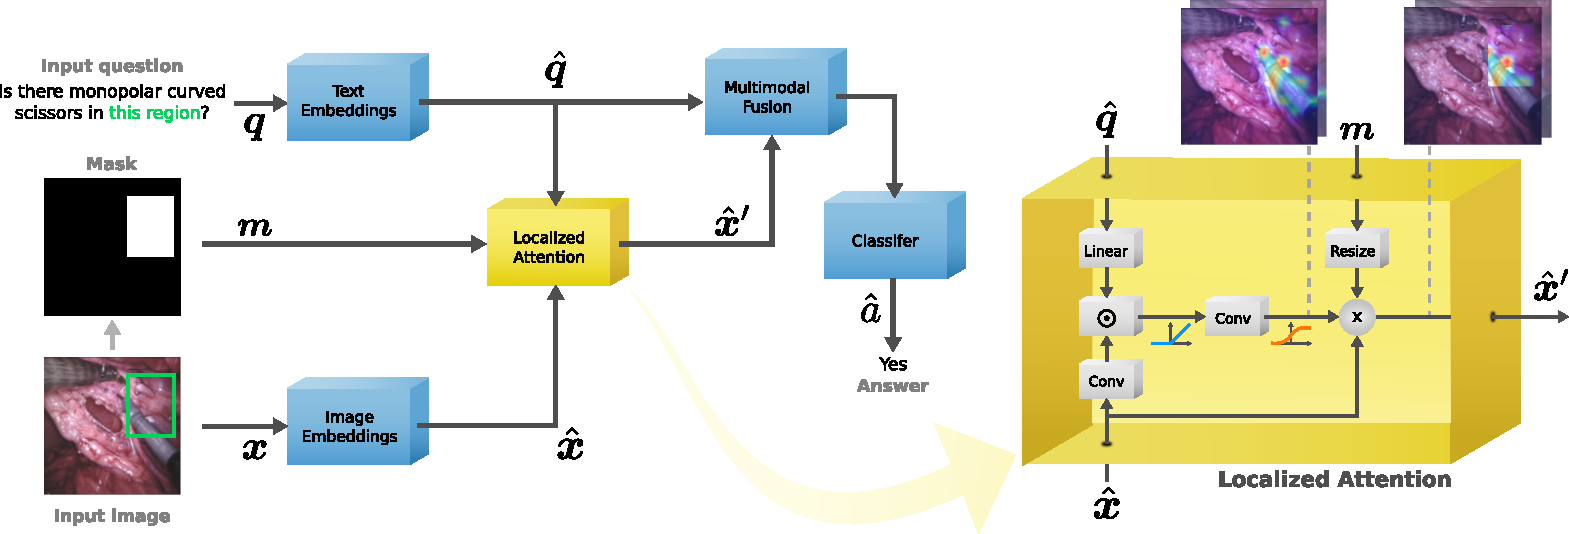
\includegraphics[width=0.99\textwidth]{Figures/Part1_LocVQA/01_locatt/method_new.pdf}
\caption{\textbf{Left:} Proposed VQA architecture for localized questions. The Localized Attention module allows the region information to be integrated into the VQA while considering the context necessary to answer the question. \textbf{Right:} Localized Attention module.  
}
\label{fig:method_locvqa}
\end{center}
\end{figure}